\documentclass[12pt,a4paper]{article}
\usepackage[utf8]{inputenc}
\usepackage[turkish]{babel}
\usepackage{amsmath,amssymb,amsfonts,amsthm}
\usepackage{geometry}
\geometry{top=2.5cm,bottom=2.5cm,left=2.5cm,right=2.5cm}
\usepackage{xcolor}
\usepackage{tikz}
\usetikzlibrary{babel,arrows.meta,positioning,calc}
\usepackage{pgfplots}
\pgfplotsset{compat=1.18}
\usepackage[most]{tcolorbox}
\usepackage{hyperref}
\usepackage{caption}
\usepackage{booktabs}
\usepackage{tabularx}

% -------------------------------------------------
% style.tex – Ortak paketler ve tcolorbox tanımları
% -------------------------------------------------
\usepackage[utf8]{inputenc}
\usepackage[turkish]{babel}
\usepackage{amsmath,amssymb,amsfonts,amsthm}
\usepackage{geometry}
\geometry{top=2.5cm,bottom=2.5cm,left=2.5cm,right=2.5cm}
\usepackage{xcolor}
\usepackage{tikz,pgfplots}
\pgfplotsset{compat=1.18}
\usepackage[most]{tcolorbox}
\usepackage{hyperref}
\usepackage{caption,booktabs,tabularx}

% ---------- Renk tanımları ----------
\definecolor{purp}{RGB}{102,51,153}
\definecolor{tealblue}{RGB}{0,120,130}
\definecolor{mainblue}{RGB}{26,82,118}
\definecolor{alertred}{RGB}{180,40,40}
\definecolor{okgreen}{RGB}{34,139,34}

% ---------- Tek‑argümanlı kutular ----------
\newtcolorbox{box}[2][]{
  colback=white,
  colframe=purp,
  title={#2},
  arc=2mm,
  breakable,
  #1
}

\newtcolorbox{uyari}[1][]{
  colback=yellow!10,
  colframe=orange,
  title={Uyarı},
  arc=2mm,
  breakable,
  #1
}

% ---------- Diğer yardımcı kutular (isteğe bağlı) ----------
\newtcolorbox{ornek}[2][]{
  colback=mainblue!5!white,
  colframe=mainblue,
  title={#2},
  arc=2mm,
  breakable,
  #1
}

\newtcolorbox{odev}[2][]{
  colback=okgreen!5!white,
  colframe=okgreen,
  title={Çözümü Olmayan Ödev ve Tam Çözümü: #2},
  arc=2mm,
  breakable,
  #1
}

\newtcolorbox{tanim}[2][]{
  colback=gray!5!white,
  colframe=gray!60!black,
  title={#2},
  arc=2mm,
  breakable,
  #1
}

\newtcolorbox{sezgi}[2][]{
  colback=tealblue!5!white,
  colframe=tealblue,
  title={Sezgisel Bakış ve Basit Anlatım: #2},
  arc=2mm,
  breakable,
  #1
}

\title{\textbf{İSTATİSTİK TEORİSİ}\\[0.3em] \Large 5. Hafta Ders Notları ve Detaylı Konu Anlatımı}
\author{Ders Notları Düzenlemesi, Sezgisel Açıklamalar ve Çözümlü Analizler}
\date{}

\begin{document}
\maketitle

\begin{abstract}
Bu çalışma; İstatistik Teorisi dersinin 5. haftasında yer alan \textbf{Örnekleme Dağılımları} ($\chi^2$, Student-$t$, Fisher-$F$), \textbf{İki Değişkenli Dönüşümler ve Konvolüsyon}, \textbf{Sürekli Eşleme Teoremi (CMT)} ve \textbf{Hata Kareler Ortalaması (MSE) Optimizasyonu} konularını içermektedir. Ağır matematiksel türetimler sezgisel şemalar ve adım adım örneklerle basitleştirilmiştir.
\end{abstract}

\hrule
\vspace{1em}

\section{Büyük Resim: 5. Haftada Ne Öğreniyoruz ve Neden?}

\begin{sezgi}{Normal Dağılımın Çekirdek Ailesi ($\chi^2$, $t$ ve $F$)}
İstatistikte en sık kullandığımız testler ($t$-testi, ANOVA, Ki-Kare testi) gökten zembille inmemiştir; hepsi tek bir kaynaktan: **Standart Normal Dağılımdan ($Z \sim N(0,1)$)** türetilmiştir!
\begin{itemize}
    \item Standart normal değişkenlerin karelerini toplarsanız $\longrightarrow$ \textbf{Ki-Kare Dağılımı} ($\chi^2$) doğar.
    \item Kitle varyansı bilinmediğinde $\sigma$ yerine örneklem varyansı $S$ koyarsanız $\longrightarrow$ \textbf{Student-$t$ Dağılımı} doğar.
    \item İki farklı grubun varyanslarını birbirine oranlarsanız $\longrightarrow$ \textbf{Fisher-$F$ Dağılımı} doğar.
\end{itemize}
Haftanın ikinci kısmında ise istatistiksel tahmin edicilerin kalitesini ölçen en temel kriter olan \textbf{Hata Kareler Ortalamasını (MSE)} ve sapma-varyans dengesini (bias-variance tradeoff) öğreniriz.
\end{sezgi}

\begin{center}
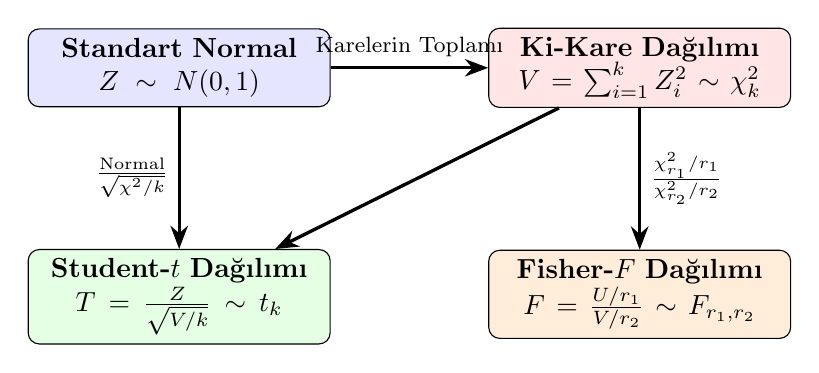
\begin{tikzpicture}[node distance=2cm, auto, >=Stealth]
    \node[draw, rounded corners, fill=blue!10, text width=3.6cm, align=center] (norm) {\textbf{Standart Normal}\\$Z \sim N(0, 1)$};
    \node[draw, rounded corners, fill=red!10, text width=3.6cm, align=center, right=2cm of norm] (chi) {\textbf{Ki-Kare Dağılımı}\\$V = \sum_{i=1}^k Z_i^2 \sim \chi^2_k$};
    \node[draw, rounded corners, fill=green!10, text width=3.6cm, align=center, below=1.8cm of norm] (t) {\textbf{Student-$t$ Dağılımı}\\$T = \frac{Z}{\sqrt{V/k}} \sim t_k$};
    \node[draw, rounded corners, fill=orange!15, text width=3.6cm, align=center, below=1.8cm of chi] (f) {\textbf{Fisher-$F$ Dağılımı}\\$F = \frac{U/r_1}{V/r_2} \sim F_{r_1, r_2}$};

    \draw[->, very thick] (norm) -- node[above, font=\footnotesize]{Karelerin Toplamı} (chi);
    \draw[->, very thick] (norm) -- node[left, font=\footnotesize]{$\frac{\text{Normal}}{\sqrt{\chi^2/k}}$} (t);
    \draw[->, very thick] (chi) -- (t);
    \draw[->, very thick] (chi) -- node[right, font=\footnotesize]{$\frac{\chi^2_{r_1}/r_1}{\chi^2_{r_2}/r_2}$} (f);
\end{tikzpicture}
\captionof{figure}{Normal dağılımdan türetilen örnekleme dağılımları arasındaki hiyerarşik ilişkiler.}
\end{center}

---

\section{Örnekleme Dağılımları (Sampling Distributions)}

\subsection{1. Standart Normalin Karesi ve \texorpdfstring{$\chi^2_1$}{Ki-kare(1)} Dağılımı}

\begin{tanim}{Teorem: $Z \sim N(0, 1) \implies Y = Z^2 \sim \chi^2_1$}
$Z \sim N(0, 1)$ olsun. $Y = Z^2$ karesel dönüşümünün dağılım fonksiyonu simetriden $F_Y(y) = P(Z^2 \le y) = 2F_Z(\sqrt{y}) - 1$'dir ($y > 0$).  
Türevi alınırsa:
\begin{equation}
    f_Y(y) = 2 f_Z(\sqrt{y}) \frac{1}{2\sqrt{y}} = \frac{1}{\sqrt{y}} \frac{1}{\sqrt{2\pi}} e^{-y/2} = \frac{1}{2^{1/2} \Gamma(1/2)} y^{1/2 - 1} e^{-y/2}
\end{equation}
Bu yoğunluk $k=1$ serbestlik dereceli \textbf{Ki-Kare ($\chi^2_1$)} dağılımıdır.
\end{tanim}

\subsection{2. Bağımsız Ki-Karelerin Toplamı}

$Z_i \overset{\text{i.i.d.}}{\sim} N(0, 1)$ ise $X_i = Z_i^2 \sim \chi^2_1$ değişkeninin MÇF'si:
\begin{equation}
    M_{X_i}(t) = \int_{-\infty}^{\infty} e^{tz^2} \frac{1}{\sqrt{2\pi}} e^{-z^2/2} dz = \frac{1}{\sqrt{2\pi}} \int_{-\infty}^{\infty} e^{-\frac{z^2}{2}(1 - 2t)} dz = (1 - 2t)^{-1/2}
\end{equation}
Bağımsız $k$ tanesinin toplamı $Y = \sum_{i=1}^k Z_i^2$ için MÇF:
\begin{equation}
    M_Y(t) = \prod_{i=1}^k M_{X_i}(t) = \left[ (1 - 2t)^{-1/2} \right]^k = (1 - 2t)^{-k/2} \implies \boxed{Y = \sum_{i=1}^k Z_i^2 \sim \chi^2_k}
\end{equation}

\subsection{3. Örneklem Varyansının Dağılımı: \texorpdfstring{$\frac{(n-1)S^2}{\sigma^2} \sim \chi^2_{n-1}$}{(n-1)S^2/sigma^2 ~ Ki-kare(n-1)}}

$X_i \overset{\text{i.i.d.}}{\sim} N(\mu, \sigma^2)$ olsun. Cebirsel toplam kareler özdeşliğini yazalım:
\begin{equation}
    \sum_{i=1}^n (X_i - \mu)^2 = \sum_{i=1}^n (X_i - \bar{X})^2 + n(\bar{X} - \mu)^2
\end{equation}
Her iki tarafı kitle varyansı $\sigma^2$'ye bölelim:
\begin{equation}
    \underbrace{\sum_{i=1}^n \left(\frac{X_i - \mu}{\sigma}\right)^2}_{A \sim \chi^2_n} = \underbrace{\frac{(n-1)S^2}{\sigma^2}}_{B} + \underbrace{\left(\frac{\bar{X} - \mu}{\sigma/\sqrt{n}}\right)^2}_{C \sim \chi^2_1}
\end{equation}
Normal kitlelerde örneklem ortalaması ($\bar{X}$) ile örneklem varyansı ($S^2$) istatistiksel olarak \textbf{bağımsızdır} (Basu / Cochran teoremi). Dolayısıyla $B$ ile $C$ bağımsızdır:
\begin{equation}
    M_A(t) = M_B(t) \cdot M_C(t) \implies M_B(t) = \frac{M_A(t)}{M_C(t)} = \frac{(1 - 2t)^{-n/2}}{(1 - 2t)^{-1/2}} = (1 - 2t)^{-\frac{n-1}{2}}
\end{equation}
Teklik teoremi gereğince:
\begin{equation}
    \boxed{\frac{(n-1)S^2}{\sigma^2} \sim \chi^2_{n-1}}
\end{equation}
\textit{Sezgisel Anlamı:} Serbestlik derecesi $n$ değil $n-1$'dir; çünkü örneklem ortalaması $\bar{X}$ tahmin edildiğinde 1 serbestlik derecesi (bilgi) harcanmıştır!

---

\section{\texorpdfstring{Student-$t$}{Student-t} ve \texorpdfstring{Fisher-$F$}{Fisher-F} Dağılımlarının Türetilmesi}

\subsection{1. \texorpdfstring{Student-$t$}{Student-t} Dağılımının Jacobiyen İle Türetimi}

\begin{tanim}{Student-$t$ Dağılımı}
$Z \sim N(0, 1)$ ve $V \sim \chi^2_r$ bağımsız iki değişken olsun.  
\begin{equation}
    T = \frac{Z}{\sqrt{V/r}}
\end{equation}
değişkenine $r$ serbestlik dereceli \textbf{Student-$t$} dağılımı denir ($T \sim t_r$).
\end{tanim}

\textbf{Türetim Adımları:}  
$T = \frac{Z}{\sqrt{V/r}}$ ve $U = V$ dönüşümü yapalım:
\begin{equation}
    z = t \sqrt{u/r}, \quad v = u \implies |J| = \left| \begin{matrix} \sqrt{u/r} & \frac{t}{2\sqrt{ur}} \\ 0 & 1 \end{matrix} \right| = \sqrt{\frac{u}{r}}
\end{equation}
Bileşik yoğunluk $f(t, u) = f_Z(z(t, u)) f_V(u) |J|$:
\begin{equation}
    f(t, u) = \frac{1}{\sqrt{2\pi}} \frac{1}{2^{r/2}\Gamma(r/2)} u^{r/2 - 1} \exp\left( -\frac{u}{2}\left( 1 + \frac{t^2}{r} \right) \right) u^{1/2} r^{-1/2}
\end{equation}
$u \in (0, \infty)$ üzerinden Gamma integrali ($\int_0^\infty u^{\alpha-1} e^{-\beta u} du = \frac{\Gamma(\alpha)}{\beta^\alpha}$) ile marjinal yoğunluk hesaplanırsa:
\begin{equation}
    \boxed{f(t) = \frac{\Gamma\left(\frac{r+1}{2}\right)}{\sqrt{r\pi} \, \Gamma\left(\frac{r}{2}\right)} \left( 1 + \frac{t^2}{r} \right)^{-\frac{r+1}{2}}, \quad -\infty < t < \infty}
\end{equation}

\begin{center}
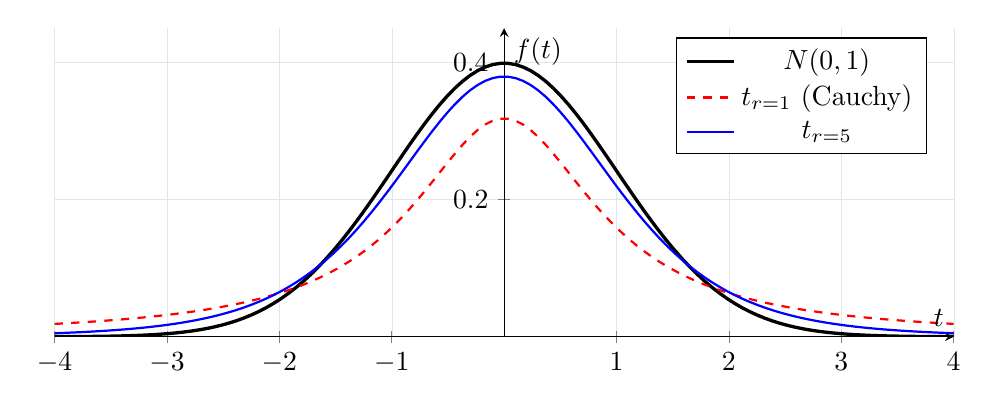
\begin{tikzpicture}
\begin{axis}[
    width=13cm, height=5.5cm,
    axis lines=center,
    xlabel={$t$}, ylabel={$f(t)$},
    xmin=-4, xmax=4, ymin=0, ymax=0.45,
    samples=120, domain=-4:4,
    legend pos=north east,
    grid=both, grid style={line width=.1pt, draw=gray!20}
]
    \addplot[black, very thick] {1/sqrt(2*pi) * exp(-x^2/2)};
    \addlegendentry{$N(0, 1)$}

    \addplot[red, thick, dashed] {1/(pi * (1 + x^2))};
    \addlegendentry{$t_{r=1}$ (Cauchy)}

    \addplot[blue, thick] {0.3796 * (1 + x^2/5)^(-3)};
    \addlegendentry{$t_{r=5}$}
\end{axis}
\end{tikzpicture}
\captionof{figure}{Student-$t$ dağılımlarının Normal dağılımla karşılaştırması ($r \to \infty$ iken $t_r \xrightarrow{d} N(0, 1)$, $r=1$ iken Cauchy dağılımıdır).}
\end{center}

\subsection{2. \texorpdfstring{Fisher-$F$}{Fisher-F} Dağılımının Türetimi}

\begin{tanim}{Fisher-$F$ Dağılımı}
$U \sim \chi^2_{r_1}$ ve $V \sim \chi^2_{r_2}$ bağımsız iki ki-kare değişkeni olsun.
\begin{equation}
    W = \frac{U / r_1}{V / r_2}
\end{equation}
oranına $r_1$ ve $r_2$ serbestlik dereceli \textbf{Snedecor-Fisher $F$} dağılımı denir ($W \sim F_{r_1, r_2}$).
\end{tanim}
Jacobiyen dönüşümü yapılıp marjinal integral alındığında:
\begin{equation}
    \boxed{f(w) = \frac{\Gamma\left(\frac{r_1 + r_2}{2}\right)}{\Gamma\left(\frac{r_1}{2}\right) \Gamma\left(\frac{r_2}{2}\right)} \left(\frac{r_1}{r_2}\right)^{r_1/2} \frac{w^{\frac{r_1}{2} - 1}}{\left(1 + \frac{r_1}{r_2}w\right)^{\frac{r_1+r_2}{2}}}, \quad w > 0}
\end{equation}

---

\section{İki Değişkenli Dönüşümler ve Konvolüsyon}

\begin{tanim}{Konvolüsyon İntegrali (Toplamın Yoğunluğu)}
$X$ ve $Y$ bağımsız sürekli rastgele değişkenler olsun. Toplamları olan $U = X + Y$ değişkeninin olasılık yoğunluk fonksiyonu:
\begin{equation}
    f_U(u) = (f_X * f_Y)(u) = \int_{-\infty}^{\infty} f_X(v) \, f_Y(u - v) \, dv
\end{equation}
\end{tanim}

\begin{ornek}{Örnek 1: $f(x) = 2x, \; 0 < x < 1$ İçin $Y = X_1 + X_2$'nin Dağılımı}
$f(x_1, x_2) = 4x_1 x_2$. $Y_1 = X_1 + X_2, Y_2 = X_2 \implies |J| = 1$.  
Sınırlar: $0 < y_1 - y_2 < 1$ ve $0 < y_2 < 1$.
\begin{itemize}
    \item \textbf{Bölge I ($0 < y_1 < 1$):} $y_2 \in (0, y_1)$
    \begin{equation}
        f(y_1) = \int_{0}^{y_1} 4(y_1 y_2 - y_2^2) dy_2 = \left[ 2y_1 y_2^2 - \frac{4}{3}y_2^3 \right]_0^{y_1} = \boxed{\frac{2}{3}y_1^3}
    \end{equation}
    \item \textbf{Bölge II ($1 \le y_1 < 2$):} $y_2 \in (y_1 - 1, 1)$
    \begin{equation}
        f(y_1) = \int_{y_1 - 1}^{1} 4(y_1 y_2 - y_2^2) dy_2 = \boxed{\frac{2}{3}\left( -y_1^3 + 6y_1 - 4 \right)}
    \end{equation}
\end{itemize}
\end{ornek}

\begin{ornek}{Örnek 2: Üçgensel Dağılım ($Y = X_2 - X_1$)}
$f(x_1, x_2) = 1/2, \; x_1 + x_2 < 2, \; x_1, x_2 > 0$ bölgesinde $Y = X_2 - X_1$ dönüşümü:
\begin{equation}
    f_Y(y) = \frac{2 - |y|}{4}, \quad -2 < y < 2
\end{equation}
şeklinde simetrik bir üçgensel dağılım üretir.
\end{ornek}

\begin{center}
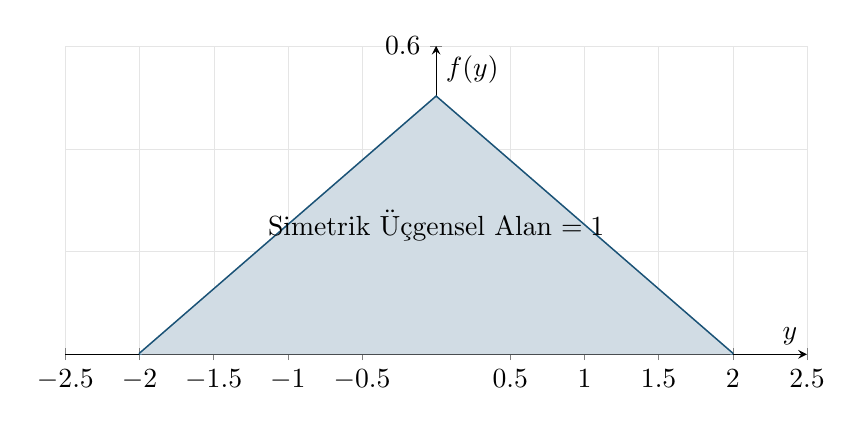
\begin{tikzpicture}
\begin{axis}[
    width=11cm, height=5.5cm,
    axis lines=center,
    xlabel={$y$}, ylabel={$f(y)$},
    xmin=-2.5, xmax=2.5, ymin=0, ymax=0.6,
    grid=both, grid style={line width=.1pt, draw=gray!20}
]
    \addplot[mainblue, very thick] coordinates {(-2, 0) (0, 0.5) (2, 0)};
    \addplot[fill=mainblue!20, draw=none] coordinates {(-2, 0) (0, 0.5) (2, 0)} \closedcycle;
    \node at (axis cs:0, 0.25) {Simetrik Üçgensel Alan $= 1$};
\end{axis}
\end{tikzpicture}
\captionof{figure}{$Y = X_2 - X_1$ değişkeninin simetrik üçgensel olasılık yoğunluk fonksiyonu.}
\end{center}

---

\section{5. Hafta Ödevi ve Eksiksiz Çözümü}

\begin{odev}{Sürekli Eşleme Teoremi (Continuous Mapping Theorem - CMT)}
\textbf{Ödev Sorusu (Sayfa 35):} $g: \mathbb{R} \to \mathbb{R}$ fonksiyonu sürekli olsun. $\hat{\theta}_n \xrightarrow{P} \theta$ ise:
\begin{equation}
    g(\hat{\theta}_n) \xrightarrow{P} g(\theta)
\end{equation}
olduğunu ispatlayınız. *(Notlarda "İspatı ödev..." olarak bırakılmıştır).*

\bigskip
\textbf{Adım Adım Detaylı İspat:}
Göstermemiz gereken matematiksel hedef:
\begin{equation}
    \forall \epsilon > 0 \quad \text{için} \quad \lim_{n \to \infty} P\left( |g(\hat{\theta}_n) - g(\theta)| \ge \epsilon \right) = 0
\end{equation}
\begin{enumerate}
    \item Herhangi bir $\epsilon > 0$ sabitlensin.
    \item $g$ fonksiyonu $\theta$ noktasında sürekli olduğundan analizin $\epsilon-\delta$ tanımı gereği:
    \begin{equation}
        |x - \theta| < \delta \implies |g(x) - g(\theta)| < \epsilon
    \end{equation}
    olacak şekilde bir $\delta > 0$ sayısı mevcuttur.
    \item Mantık kurallarına göre $(P \implies Q) \iff (\neg Q \implies \neg P)$ karşıt-tersi denktir:
    \begin{equation}
        |g(x) - g(\theta)| \ge \epsilon \implies |x - \theta| \ge \delta
    \end{equation}
    \item Bu bağıntı rastgele değişkenlerin olay kümeleri için bir alt küme ilişkisi tanımlar:
    \begin{equation}
        \left\{ \omega : |g(\hat{\theta}_n(\omega)) - g(\theta)| \ge \epsilon \right\} \subseteq \left\{ \omega : |\hat{\theta}_n(\omega) - \theta| \ge \delta \right\}
    \end{equation}
    \item Olasılık ölçüsünün monotonluğundan ($A \subseteq B \implies P(A) \le P(B)$):
    \begin{equation}
        P\left( |g(\hat{\theta}_n) - g(\theta)| \ge \epsilon \right) \le P\left( |\hat{\theta}_n - \theta| \ge \delta \right)
    \end{equation}
    \item Hipotez gereği $\hat{\theta}_n \xrightarrow{P} \theta$ olduğundan sabit $\delta > 0$ için sağ taraf sıfıra gider:
    \begin{equation}
        \lim_{n \to \infty} P\left( |\hat{\theta}_n - \theta| \ge \delta \right) = 0
    \end{equation}
    \item Sandviç Teoremi gereğince:
    \begin{equation}
        0 \le \lim_{n \to \infty} P\left( |g(\hat{\theta}_n) - g(\theta)| \ge \epsilon \right) \le 0 \implies \boxed{g(\hat{\theta}_n) \xrightarrow{P} g(\theta)}
    \end{equation}
\end{enumerate}
\end{odev}

---

\section{Hata Kareler Ortalaması (MSE) ve Optimal Tahmin}

\begin{tanim}{Hata Kareler Ortalaması (Mean Squared Error - MSE)}
Bir $\theta$ parametresinin tahmin edicisi $\hat{\theta}$ olsun.
\begin{equation}
    \boxed{\text{MSE}_\theta(\hat{\theta}) = E\left[ (\hat{\theta} - \theta)^2 \right] = V(\hat{\theta}) + \left[ \text{Bias}(\hat{\theta}) \right]^2}
\end{equation}
\end{tanim}

\begin{sezgi}{Yansızlık mı, Düşük MSE mi? (Bias-Variance Tradeoff)}
Geleneksel olarak tahmin edicinin ortalamasının kitle parametresine eşit olması istenir ($E(\hat{\theta})=\theta$, Yansızlık / Unbiasedness).  
Ancak bir tahmin edici yansız olsa bile varyansı (savrulması) çok büyük olabilir!  
Bazen birazcık yanlılığa (bias) izin vermek varyansı öyle muazzam düşürür ki, toplam hata karesi (MSE) çok daha küçük kalır. Modern istatistik ve yapay zekanın (Ridge Regresyon vb.) kalbinde bu ilke yatar.
\end{sezgi}

\begin{ornek}{Örnek 3: Normal Dağılımda $\sigma^2$ İçin En Küçük MSE'li Tahmin Edici}
$T = \sum_{i=1}^n (X_i - \bar{X})^2 \sim \sigma^2 \chi^2_{n-1}$ olsun. $\hat{\sigma}^2 = a T$ biçimindeki tahmin ediciler arasında MSE'yi minimize eden $a$ değerini bulunuz.

\bigskip
\textbf{Çözüm:}
$E(T) = (n-1)\sigma^2$ ve $V(T) = 2(n-1)\sigma^4$.
\begin{align}
    \text{MSE}(aT) &= V(aT) + [E(aT) - \sigma^2]^2 = a^2 2(n-1)\sigma^4 + [a(n-1)\sigma^2 - \sigma^2]^2 \notag \\
    &= \sigma^4 \left[ 2(n-1)a^2 + ((n-1)a - 1)^2 \right]
\end{align}
$a$'ya göre türev alıp sıfıra eşitleyelim:
\begin{equation}
    \frac{d}{da} \text{MSE}(aT) = \sigma^4 \left[ 4(n-1)a + 2(n-1)((n-1)a - 1) \right] = 0
\end{equation}
$2(n-1)$ çarpanını sadeleştirelim ($n > 1$):
\begin{equation}
    2a + (n-1)a - 1 = 0 \implies a(n + 1) = 1 \implies \boxed{a = \frac{1}{n+1}}
\end{equation}
\textbf{Çarpıcı Sonuç:}
\begin{itemize}
    \item Klasik yansız tahmin edici: $S^2 = \frac{T}{n-1}$
    \item En küçük MSE'ye sahip tahmin edici: $\hat{\sigma}^2_{\text{MSE}} = \frac{T}{n+1}$
\end{itemize}
$n+1$'e bölünen tahmin edici yansız değildir (bir miktar sapmalıdır); ancak varyansı çok daha küçük olduğu için ortalama hata karesi (MSE) $S^2$'den daha düşüktür!
\end{ornek}

\begin{center}
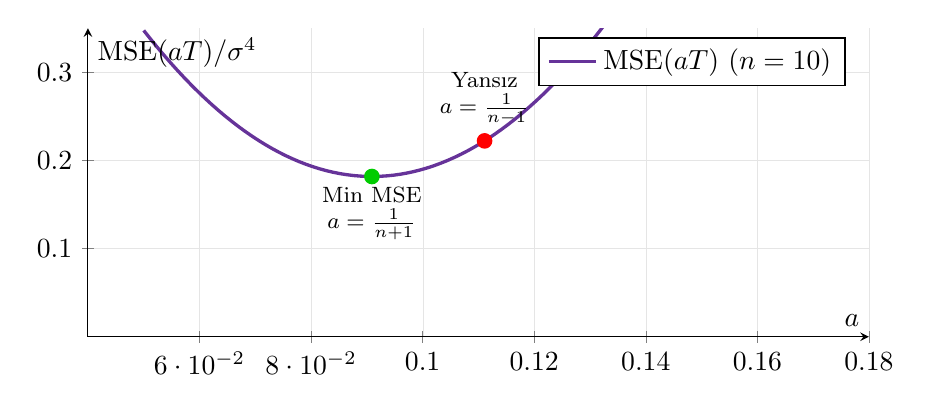
\begin{tikzpicture}
\begin{axis}[
    width=11.5cm, height=5.5cm,
    axis lines=center,
    xlabel={$a$}, ylabel={$\text{MSE}(aT) / \sigma^4$},
    xmin=0.04, xmax=0.18, ymin=0, ymax=0.35,
    samples=100, domain=0.05:0.17,
    legend pos=north east,
    grid=both, grid style={line width=.1pt, draw=gray!20}
]
    \addplot[purp, very thick] {99*x^2 - 18*x + 1};
    \addlegendentry{$\text{MSE}(aT)$ ($n=10$)}

    \node[circle, fill=green!80!black, inner sep=2pt] at (axis cs:0.0909, 0.1818) {};
    \node at (axis cs:0.0909, 0.14) [font=\footnotesize, align=center] {Min MSE\\$a = \frac{1}{n+1}$};

    \node[circle, fill=red, inner sep=2pt] at (axis cs:0.1111, 0.2222) {};
    \node at (axis cs:0.1111, 0.27) [font=\footnotesize, align=center] {Yansız\\$a = \frac{1}{n-1}$};
\end{axis}
\end{tikzpicture}
\captionof{figure}{$n=10$ için MSE parabolü. $a=\frac{1}{n+1}$ noktasında MSE global minimum yapar.}
\end{center}

\vspace{0.5em}
\section{5. Hafta Hızlı Tekrar ve Formül Tablosu}

\begin{table}[ht]
\centering
\small
\renewcommand{\arraystretch}{1.35}
\begin{tabularx}{\textwidth}{@{}l l X@{}}
\toprule
\textbf{Dağılım / Teorem} & \textbf{Tanım ve Formül} & \textbf{Pratik Anlamı / Kullanım Alanı} \\ \midrule
\textbf{Ki-Kare ($\chi^2_k$)} & $\sum_{i=1}^k Z_i^2, \quad Z_i \sim N(0,1)$ & Standart normallerin kareler toplamı; varyans testlerinin temeli. \\
\textbf{Örneklem Varyansı} & $\frac{(n-1)S^2}{\sigma^2} \sim \chi^2_{n-1}$ & Normal kitlede $S^2$'nin kitle varyansına oranı $n-1$ serbestlikli ki-karedir. \\
\textbf{Student-$t_r$} & $\frac{Z}{\sqrt{V/r}}, \quad Z \sim N(0,1), V \sim \chi^2_r$ & Kitle varyansı $\sigma$ bilinmediğinde ortalama testleri ($t$-testi). \\
\textbf{Fisher-$F_{r_1, r_2}$} & $\frac{U/r_1}{V/r_2}, \quad U \sim \chi^2_{r_1}, V \sim \chi^2_{r_2}$ & İki bağımsız varyansın karşılaştırılması (ANOVA testi). \\
\textbf{CMT Teoremi} & $\hat{\theta}_n \xrightarrow{P} \theta \implies g(\hat{\theta}_n) \xrightarrow{P} g(\theta)$ & Sürekli fonksiyonlar olasılıkta yakınsamayı korur. \\
\textbf{MSE Ayrışımı} & $\text{MSE}(\hat{\theta}) = V(\hat{\theta}) + \text{Bias}^2$ & Sapma ile varyans arasındaki değiş-tokuş kriteri. \\ \bottomrule
\end{tabularx}
\caption{5. Haftanın Temel Örnekleme Dağılımları, Dönüşümleri ve Tahmin Kriterleri}
\end{table}

\end{document}
